\documentclass[12pt,a4paper]{article}

% ==== 导言区 ====
%================================
% note-setup-leftsidebox.tex
% fenglielie@qq.com 2025-09-12
%================================

\usepackage{amsmath,amsthm,amsfonts,amssymb}
\usepackage{mathtools}
\usepackage{mathrsfs}
\usepackage{bm}
\usepackage{extarrows}
\usepackage[a4paper, margin=1in]{geometry}
\usepackage{float}
\usepackage{indentfirst}
\usepackage{anyfontsize}
\usepackage{booktabs,multirow,multicol}
\usepackage[shortlabels,inline]{enumitem}
\usepackage{appendix}

\usepackage[dvipsnames]{xcolor}
\usepackage{graphicx}
\graphicspath{
    {./figure/}{./figures/}{./image/}{./images/}{./graphic/}{./graphics/}{./picture/}{./pictures/}
}
\usepackage{subcaption}
% TikZ-cd: commutative diagrams (loads tikz)
\usepackage{tikz-cd}
% Optional: enable additional tikz libraries if you need advanced arrow styles
\usetikzlibrary{arrows.meta,decorations.pathmorphing,cd}

\usepackage[ruled,linesnumbered,noline]{algorithm2e}
\usepackage{listings}
\lstdefinestyle{simpleStyle}{
    basicstyle=\ttfamily\small,
    breaklines=true,
    keywordstyle=\color{blue},
    identifierstyle=\color{black},
    stringstyle=\color{violet},
    commentstyle=\color[RGB]{34,139,34},
    showstringspaces=false,
    numbers=left,
    numbersep=2em,
    numberstyle=\footnotesize,
    frame=single,
    framesep=1em,
}
\lstset{style=simpleStyle}

\usepackage{hyperref}
\hypersetup{
    colorlinks=true,linkcolor=,urlcolor=cyan
}

\renewcommand*{\proofname}{\normalfont\bfseries Proof}

\usepackage{thmtools}

%% define environments
\declaretheorem[style=plain, name=Theorem, numbered=yes, numberwithin=section]{theoremplain}
\declaretheorem[style=plain, name=Proposition, numbered=yes, sibling=theoremplain]{propositionplain}
\declaretheorem[style=plain, name=Corollary, numbered=yes, sibling=theoremplain]{corollaryplain}
\declaretheorem[style=plain, name=Definition, numbered=yes, sibling=theoremplain]{definitionplain}


\declaretheorem[style=plain, name=Theorem, numbered=yes, numberwithin=section]{theorem}
\declaretheorem[style=plain, name=Theorem, numbered=no]{theorem*}

\declaretheorem[style=plain, name=Proposition, numbered=yes, sibling=theorem]{proposition}
\declaretheorem[style=plain, name=Proposition, numbered=no]{proposition*}

\declaretheorem[style=plain, name=Corollary, numbered=yes, sibling=theorem]{corollary}
\declaretheorem[style=plain, name=Corollary, numbered=no]{corollary*}

\declaretheorem[style=plain, name=Lemma, numbered=yes, sibling=theorem]{lemma}
\declaretheorem[style=plain, name=Lemma, numbered=no]{lemma*}

\declaretheorem[style=plain, name=Claim, numbered=yes, sibling=theorem]{claim}
\declaretheorem[style=plain, name=Claim, numbered=no]{claim*}

\declaretheorem[style=definition, name=Definition, numbered=yes, numberwithin=section]{definition}
\declaretheorem[style=definition, name=Definition, numbered=no]{definition*}

\declaretheorem[style=definition, name=Example, numbered=yes, numberwithin=section]{example}
\declaretheorem[style=definition, name=Example, numbered=no]{example*}

\declaretheorem[style=definition, name=Problem, numbered=yes, numberwithin=section]{problem}
\declaretheorem[style=definition, name=Problem, numbered=no]{problem*}

\declaretheorem[style=remark, name=Remark, numbered=yes, numberwithin=section]{remark}
\declaretheorem[style=remark, name=Remark, numbered=no]{remark*}

\declaretheorem[style=remark, name=Note, numbered=yes, numberwithin=section]{note}
\declaretheorem[style=remark, name=Note, numbered=no]{note*}

\declaretheoremstyle[headfont=\bfseries, bodyfont=\normalfont, spaceabove=3pt, spacebelow=3pt, qed=\ensuremath{\square}]{solutionstyle}

\declaretheorem[style=solutionstyle, name=Solution, numbered=yes, numberwithin=section]{solution}
\declaretheorem[style=solutionstyle, name=Solution, numbered=no]{solution*}

\usepackage[most]{tcolorbox}

\newcommand{\newtcbenvironment}[2]{
    \tcolorboxenvironment{#1}{#2, enhanced, breakable, sharp corners,leftrule=2pt, rightrule=0pt, toprule=0pt, bottomrule=0pt}
    \tcolorboxenvironment{#1*}{#2, enhanced, breakable, rounded corners,leftrule=2pt, rightrule=0pt, toprule=0pt, bottomrule=0pt}
}

%% define styles

\newtcbenvironment{theorem}{colframe=RoyalPurple, colback=RoyalPurple!8}
\newtcbenvironment{proposition}{colframe=RoyalPurple, colback=RoyalPurple!8}
\newtcbenvironment{corollary}{colframe=NavyBlue, colback=SkyBlue!8}
\newtcbenvironment{lemma}{colframe=NavyBlue, colback=SkyBlue!8}
\newtcbenvironment{claim}{colframe=NavyBlue, colback=SkyBlue!8}

\newtcbenvironment{definition}{colframe=ForestGreen, colback=ForestGreen!5}
\newtcbenvironment{example}{colframe=RawSienna, colback=RawSienna!5}
\newtcbenvironment{problem}{colframe=WildStrawberry!30, colback=WildStrawberry!5}

%% cbox
\newtcolorbox{cbox}[1][]{%
    enhanced,
    breakable,
    sharp corners,
    leftrule=2pt, rightrule=0pt, toprule=0pt, bottomrule=0pt,
    colframe=SkyBlue,
    colback=SkyBlue!8,
    #1
}

%% cover
\usepackage{titling}
\newcommand{\extrainfo}{}
\renewcommand{\extrainfo}[1]{\renewcommand{\extrainfocontent}{#1}}
\newcommand{\extrainfocontent}{}
\newcommand{\makecover}[1]{%
    \begin{titlepage}
    \newgeometry{margin=0in}
    \parindent=0pt
    \includegraphics[width=\linewidth]{#1} % size = 1280*1024
    \vfill
    \begin{center}
        \parbox{0.618\textwidth}{%
            \raggedleft{\bfseries \Huge \thetitle} \\[0.6pt]
            \rule{0.618\textwidth}{4pt} \\
        }
    \end{center}
    \vfill
    \begin{center}
        \parbox{0.618\textwidth}{%
          \raggedleft\Large
            \begin{tabular}{r}
                \theauthor \\
                \thedate \\
            \end{tabular}%
        }
    \end{center}
    \vfill
    \begin{center}
        \parbox[t]{0.7\textwidth}{\centering \itshape \extrainfocontent}
    \end{center}
    \vfill
    \end{titlepage}
    \restoregeometry
    \thispagestyle{empty}
}
% USAGE
% \extrainfo{xxx}
% \makecover{/path/to/cover.png}

%记号定义
\newcommand{\nn}{\mathbb{N}}
\newcommand{\zz}{\mathbb{Z}}
\newcommand{\qq}{\mathbb{Q}}
\newcommand{\rr}{\mathbb{R}}
\newcommand{\cc}{\mathbb{C}}
\newcommand{\ff}{\mathbb{F}}
\newcommand{\ffp}{\mathbb{F}_p}
\newcommand{\sph}{\mathbb{S}}
\newcommand{\Log}{\operatorname{Log}} % 调用你上传的 setup.tex 文件
% 或者你也可以直接把 setup.tex 的内容复制粘贴在这里

\title{\LaTeX{} Note Template}
\author{X}
\date{\today}

\extrainfo{Github: \href{https://github.com/Baudelaireee/Notebook}{https://github.com/Baudelaireee/Notebook}}
\begin{document}

% \maketitle
\makecover{cover/tu.jpg}
\tableofcontents
\newpage 

\section{Universal property}
Universal property is a core concept in modern mathematics, it means the same properties but appears in different objects, in the language of category theory, it means the same diagram commutative in different categories. this section is to introduce some common universal properties from set theory to group theory and topology, it can be seen as a review of basic mathematics, and a good inviation for category theory.

\subsection{Quotient}

quotient is a method to see two different things as the same things via an equivalence relation: Let \(X\) be a non-empty set and \(\sim\) be an realtion on \(X\), if it satisfies
\begin{itemize}
    \item reflexive: \(x \sim x\)
    \item symmetric: \(x \sim y \Rightarrow y \sim x    \)
    \item transitive: \(x \sim y, y \sim z \Rightarrow x \sim z\)
\end{itemize}
Then we define \(\sim\) is an \textbf{ equivalence relation} on \(X\). So we can define the equivalence class of some element \(a\) of the set as 
\[[a] = \{x \in X | x \sim a\}\]
then the \textbf{quoitent set} of \(X\) with respect to \(\sim\) is defined as
\[X/\sim := \{[a]| a \in X\}\]
but it is not the unique method to define quotient, the follwing statement gives different view.

\begin{lemma}
    Let \(X\) be a non-empty set, then the following statements are equivalent:\\

    (1) There is an equivalence relation \(\sim\) on \(X\).\\

    (2) There is a surjective map \(f: X \to Y\) to some set \(Y\).\\

    (3) There is a partition of \(X\), i.e. a family \(P = \{A_i| i\in I, A_i \subset X\}\) such that the set can be written as the disjoint union of the family
    \[X = \bigsqcup_{i \in I} A_i\]
\end{lemma}
\begin{proof}
    (1) \(\Rightarrow\) (2): Let \(Y = X/\sim\) and define \(\pi: X \to Y, x \mapsto [x]\), then it is easy to see that \(\pi\) is a surjective map.\\

    (1) \(\Rightarrow\) (3): it is equivalent to prove that the equivalence class \([x]\) and \([y]\) is disjoint if \(x \nsim y\), otherwise they are equal.\\

    (2) \(\Rightarrow\) (1): Define a relation on \(X\) by
    \[x \sim_f y \iff f(x) = f(y)\]
    It is a equivalence relation, and the equivlence class can be denoted by pre-image 
    \[[x] = f^{-1}(y)  \]
    where \(y = f(x)\).\\

    (3) \(\Rightarrow\) (1): Define a relation on \(X\) by 
    \[x \sim_P y \iff x\in A_i \wedge y \in A_i\]
    for some \(i \in I\), similarly the class can be denoted by
    \[[x] = A_i\]
    where \(x \in A_i\) and \(X/\sim_P = P\) actually.
\end{proof}

The application in the proof
\[\pi: X \to X/\sim, \quad x \mapsto [x]\]
is called the \textbf{quotient map}, it is a type of \textbf{natural map}, that means the definition of the map is unique and very natural. The statement (2) can be generalized to any map, not only surjective map, but the reason here I only state the surjective map is that (a) any map can be restricted to a surjective map; (b) the quotient map is surjective. 

The universal property of quotient can be explained as following: we expect two objects are the same up to isomorphism, in the sense of set theory, that means there is a bijection between two sets, but it is not easy to construct a bijection directly, or sometimes we do not need know what the bijection exactly is. Now we take a map \(f:X \to Y\), then we can \textbf{uniquely determine} a bijection between \(X/\sim_f\) and a subset of \(Y\), and the bijection is induced by \(f\) and the quotient map, the correspondece can be draw as following commutative diagram:
% https://q.uiver.app/#q=WzAsMyxbMCwwLCJYIl0sWzIsMCwiWSJdLFswLDIsIlgvXFxzaW1fZiJdLFswLDEsImYiXSxbMCwyLCJcXHBpIiwyLHsic3R5bGUiOnsiaGVhZCI6eyJuYW1lIjoiZXBpIn19fV0sWzIsMSwiXFxleGlzdHMhIFxcYmFye2Z9IiwwLHsic3R5bGUiOnsiYm9keSI6eyJuYW1lIjoiZGFzaGVkIn19fV1d
\[\begin{tikzcd}
	X && Y \\
	\\
	{X/\sim_f}
	\arrow["f", from=1-1, to=1-3]
	\arrow["\pi"', two heads, from=1-1, to=3-1]
	\arrow["{\exists! \bar{f}}", dashed, from=3-1, to=1-3]
\end{tikzcd}\]
We conclude the result of set theory as following:
\begin{theorem}[UPQ-SET] $ \\$
    Let \(X,Y\) be two empty sets and \(f:X \to Y\) a surjective map between them, then there is a unique bijection map \(\bar{f}: X/\sim_f \hookrightarrow Y\) such that \(f = \bar{f} \circ \pi\), where \(\pi: X \to X/\sim_f\) is the quotient map.
    
\end{theorem}

\begin{proof}
    The definition of \(\bar{f}\) is natural and uniquely by \(f = \bar{f} \circ \pi\), for any \([x] \in X/\sim_f\), define
    \[\bar{f}([x]) = f(x)\]
    the map is well-defined, because if \([x] = [y]\), then \(f(x) = f(y)\) by the definition of \(\sim_f\). The relation \(\sim_f\) implies injection \(\bar{f}\), surjection \(f\) implies surjection \(\bar{f}\), so we finish the proof.
\end{proof}

It is the simplest universal property of quotient, it can be generalized to other mathematics objects, but a little different, the map between two objects should preserve the structure, so the map will be some type of morphism, hence the quotient map should also be a morphism and the equivalence relation should be compatible with the structure. Let us consider the case of topological space.

In geometry view, a circle can be obtained by glueing the two endpoints of a line segment, for example we identify two endpoints of the interval \([0,1]\) by the relation \(0 \sim 1\), then we can get a quotient set \([0,1]/\sim\), but how to define the topology on the quotient set such that it is a space homemorphic to circle \(\sph^1\)? The answer is that the quotient map should preserve the topological structure, i.e. quotient topology is the smallest topology such that the quotient map is continuous.

\begin{definition}
    Let \((X,\mathcal{T})\) be a topological space and \(\sim\) be an equivalence relation on \(X\), the \textbf{quotient topology} on \(X/\sim\) is defined as 
    \[\mathcal{T}_{\sim} := \{U \subset X/\sim | \pi^{-1}(U) \in \mathcal{T}\}\]
    where \(\pi: X \to X/\sim, x \mapsto [x]\) is the quotient map.
\end{definition}

We can complete the example just now, firstly we find a surjective map
\[f: [0,1] \to \sph^1, \quad f(x) = e^{2\pi i x}\]
It is easy to see that \(0 \sim_f 1\) since \(f(0) = f(1)\), and the relation is exactly the relation we want, so we can conclude a bijection \(\bar{f}: [0,1]/\sim_f \to \sph^1\) such that \(f = \bar{f} \circ \pi\) by UPQ-SET, by the condtion that \(f\) and \(\pi\) are contionous, we can verify that \(\bar{f}\) is also continous. To see whether it is a homemorphism or not, we notice that \(\sph^1\) is a compact space, so we just need to verify thet \([0,1]/\sim_f\) is also a compact space \textbf{(a continous bijection from a compact space to a Hausdorff space is automatically a homeomorphism)}, that needs a properties of quotient space:
\begin{claim}
    Let \(X\) be a compact space and the graph of \(\sim\) be closed in \(X^2\), then quotient space \(X/\sim\) is also a compact space.
\end{claim}
\begin{proof}
    \[G = \{(a,b) \in X^2 |  a \sim b\}\]
    is the graph of \(\sim\),...
\end{proof}

So we can prove that \([0,1]/\sim_f\) is homeomorphic to \(\sph^1\) as above, and we can generalized the result to any similar case as following:
\begin{theorem}[UPQ-TOPO] $ \\$
    Let \((X,\mathcal{T})\) be a topological space and \((Y,\mathcal{J})\) be a topological space, \(f: X \to Y\) be a surjective continuous map, then there is a unique continous bijection \(\bar{f}: (X/\sim_f, \mathcal{T}_{\sim_f}) \to (Y,\mathcal{J})\) such that \(f = \bar{f} \circ \pi\), where \(\pi: X \to X/\sim_f\) is the quotient map.
\end{theorem}

\begin{proof}
    By UPQ-SET, there is a unique bijection \(\bar{f}\) such that \(f = \bar{f} \circ \pi\), now we will prove that \(\bar{f}\) is a homeomorphism. Take any open set \(U\) of \(Y\), then 
    \[f^{-1}(U) = (\bar{f} \circ \pi)^{-1}(U) = \pi^{-1}(\bar{f}^{-1}(U))\]
    since \(f\) is continous, then \(\pi^{-1}(\bar{f}^{-1}(U))\) is open in \(X\), by the definition of quotient topology, \(\bar{f}^{-1}(U)\) is open in \(X/\sim_f\), so \(\bar{f}\) is continous.
\end{proof}

\begin{remark}
    Here we can not get that \(\bar{f}\) is a homeomorphism directly, because the quotient map is not only a continous map, it is strong continous: a map 
    \(f:X \to Y\) is called \textbf{strong continous} if it satisfies
    \[U \in \mathcal{T}_Y  \iff f^{-1}(U) \in \mathcal{T}_X\]
    A example of a continous map but not strong continous is the map \(f: \rr \to \rr, x \mapsto 0\), here we take \(U=[-1,1]\), then \(f^{-1}(U) = \rr\) is open, but \(U\) is not open. 

    So in the statement of UPQ-TOPO, if we add that \(f\) is strong continous (for example, \(f\) is an open map), then \(\bar{f}\) is furthermore a homeomorphism.
\end{remark}

Finally, we study another basic object: group, Let \(G\) be a group and \(H\) be a subgroup of \(G\), then the subgroup can induces an equivalence relation (verify) on \(G\) by
\[a \sim_H b \iff a^{-1}b \in H\]
then the equivalence class can be denoted by left cosets
\[[a] = \{g \in G | a \sim_H g\} = aH\]
and the quotient set(it maybe not a group) is denoted by
\[G/H = \{aH | a \in G\}\]
and the quoitent map is
\[\pi: G \to G/H, \quad g \mapsto gH\]
if the quotient map furthermore preserves the group structure, i.e. it is a group homomorphism, then we expect for any \(g,h \in G\), \(\pi(gh) = \pi(g)\pi(h)\), i.e.
\[ghH = gHhH\]
a sufficent condition here is that \(hH = Hh\) for any \(h \in G\), that means \(H\) is a \textbf{normal subgroup}. Hence we can define the quotient group as follwoing:
\begin{definition}
    Let \(G\) be a group and \(H\) be a normal subgroup of \(G\), the \textbf{quotient group} of \(G\) with respect to \(H\) is defined as the set \(G/H\) with the multiplication
    \[(aH)(bH) := (ab)H\]
    for any \(a,b \in G\), and the group morphism \(\pi: G \to G/H, g \mapsto gH\) is called the \textbf{canonical morphism}.
\end{definition}

The group is a symmetric object, and the equivalence relation given by subgroup is a little special, the partition of \(G\) given by \(H\) is uniform:\\
We notice that the translation \(L_g: G \to G, x \mapsto gx\) is a bijection (not a group morphism unless \(g = e\)), so the restriction of \(L_g\) on any subgroup implies \(gH = L_g(H)\), that means any two left cosets(equivalence class) have the same \textbf{cardinality} as \(H\), in particular, if \(G\) is a finite group, then \(|H|\) divdes \(|G|\), this is the \textbf{Lagrange's theorem}.

Like what we do in topology and set theory, we can aslo conclude a universal property for group:
\begin{theorem}
    [UPQ-GRP] $ \\$
    Let \(G\) and \(K\) be two groups, \(H\) be a normal subgroup of \(G\), and \(\varphi: G \to K\) be a surjective group morphism, then there is a unique group isomorphism \(\bar{\varphi}: G/H \to K\) such that \(\varphi = \bar{\varphi} \circ \pi\), where \(\pi: G \to G/H\) is the canonical morphism.
\end{theorem}
\begin{proof}
    By UPQ-SET, there is a unique bijection \(\bar{\varphi}\) such that \(\varphi = \bar{\varphi} \circ \pi\), now we will prove that \(\bar{\varphi}\) is a group isomorphism. Take any \(aH,bH \in G/H\), then
    \[\bar{\varphi}((aH)(bH)) = \bar{\varphi}((ab)H) = \varphi(ab) = \varphi(a)\varphi(b) = \bar{\varphi}(aH)\bar{\varphi}(bH)\]
    so \(\bar{\varphi}\) is a group morphism, so we finish the proof.
\end{proof}

\newpage
\section{Some topology}
\subsection{Compact and Hausdorff space}

\begin{definition}
    Let \((X,\mathcal{T}) \in \mathbf{Top}\)\\

    - A family of open sets \(\{U_i\}_{i \in I}\) is called an \textbf{open cover} of \(X\) if \(X = \bigcup_{i \in I} U_i\); If \(J \subset I\), the subfamily \(\{U_j\}_{j \in J}\) is called a \textbf{subcover} of \(X\) if it is also an open cover of \(X\).\\

    - \(X\) is called a \textbf{compact  space} if every open cover of \(X\) has a finite subcover.
\end{definition}

Compactness is a nice property in topology, it is a \textbf{intrinsic} property about the topological space itself, it shows a type of "boundedness" and "finiteness"of the space in general. In mathematics, intrinsic property is a property independent of the embedding of the object, it will not change under different views.
\begin{proposition}
    Let \(X \in \mathbf{Top}\) be a topological space, and \(Y \subset X\) be a subspace of \(X\) with the induced topology, then a subset of \(Y\) is compact if and only if it is compact in \(X\).
\end{proposition}
\begin{proof}
    Let \(C \subset Y\) be a compact subset, then for any open cover \(\{U_i\}_{i \in I}\) of \(Y\), we can find a finite subcover \(\{U_{i_j}\}_{j=1}^n\) such that \(C \subset \bigcup_{j=1}^n U_{i_j}\). Since \(U_{i_j} \cap Y\) is open in \(Y\) and covers \(C\), we can find a finite subcover of \(C\) in \(X\), thus \(C\) is compact in \(X\).
\end{proof}

There are some other properties about compact space, it is very basic but useful, it is something about stability under different operations of set.
\begin{proposition}
    Let \(X \in \mathbf{Top}\)\\

    (1) \(A \subset X\) is closed, then it is compact.\\

    (2) Finite union of compact subsets is compact.\\

    (3) Finite intersection of compact subsets is compact.\\

    (4) Finite product of compact spaces is compact.
\end{proposition}
\begin{proof}
    
\end{proof}

\begin{remark}
    Notice the restriction of finiteness is important here. For (2), we can see that \(\rr = \bigcup_{n \in \nn} [-n,n]\) but \(\rr\) is not compact; for (3), a example is \((0,1] = \bigcap_{n \geq 1}[\frac{1}{n},1]\), here the countable intersection of compact sets is not compact, but it can hold if the sequence of set satisfies some condition, we will talk about it later; for (4), the inifinite product of compact space is compact in the sense of box topology, but the proof is not easy, we will discuss it in the last.
\end{remark}

Another important property of compact is the stability under continous map, a famous result in analysis is \textbf{Weierstrass theorem}: a continous function on a closed interval can always attain its maximum and minimum, it can be generalized to topology as following:
\begin{proposition}
    Let \(X,Y\in \mathbf{Top}\) be two topological spaces, and \(f: X \to Y\) be a continous map, if \(X\) is compact, then \(f(X)\) is also compact.
\end{proposition}
\begin{proof}
    
\end{proof}
\begin{remark}
    The inverse of the statement is not true, i.e. if \(A \subset Y\) is compact, then \(f^{-1}(A)\) is not necessary compact, for example consider the constant map \(f: \rr \to \rr, x \mapsto 0\), but it can not show the natural reason of the failure. 

    Let us review the definitio of continous map: a map \(f: X \to Y\) is continous if for any open set \(U \subset Y\), \(f^{-1}(U)\) is open in \(X\). Now if we just have a map \(f\) and a topological space \((Y,\mathcal{T}_{Y})\), then we can define a topology on \(X\) by \(f\) as following:
    \[\mathcal{T}_f := \{f^{-1}(U)|U \in \mathcal{T}_Y\}\]
    It is called the \textbf{pullback topology} (PLS verify), it is clearly the smallest topology sucht that \(f\) is continous. So by this view, we can rewirte the definition of the continous map as following:
    \begin{definitionplain*}
     A map \(f: X \to Y\) is continous if the topology on \(X\) is finer than the pullback topology \(\mathcal{T}_f\), i.e. \(\mathcal{T}_X \supset \mathcal{T}_f\).
    \end{definitionplain*}
    Hence we can conlude the reason: if a topology is very fine (like discrete topology), then a subset will be difficult to be compact, but the continous map says that the topology on \(X\) will be at least fine as the pullback topology, so the inverse image of a compact set may not be compact if the pullback is very fine.\\

    However, compactness is not a sufficent condition in many cases. For example, we always talk about the compact set in a metric space, but not all the topological space is metrizable, so another topogical properties is needed here.

    \begin{definition}
        A topological space \((X,\mathcal{T})\) is called a \textbf{Hausdorff space} if for any two different points \(x,y \in X\), there are two open sets \(U,V \in \mathcal{T}\) such that
        \[x \in U, y \in V, U \cap V = \emptyset\]
    \end{definition}
    A typical example of non-Hausdorff space is the a two-point space:
    \[X=\{a,b\},\quad \mathcal{T}=\{X,\emptyset,\{a\}\}\]
    Intuitively, it can be drawed by venus graph:
    \begin{figure}[H]
        \centering
        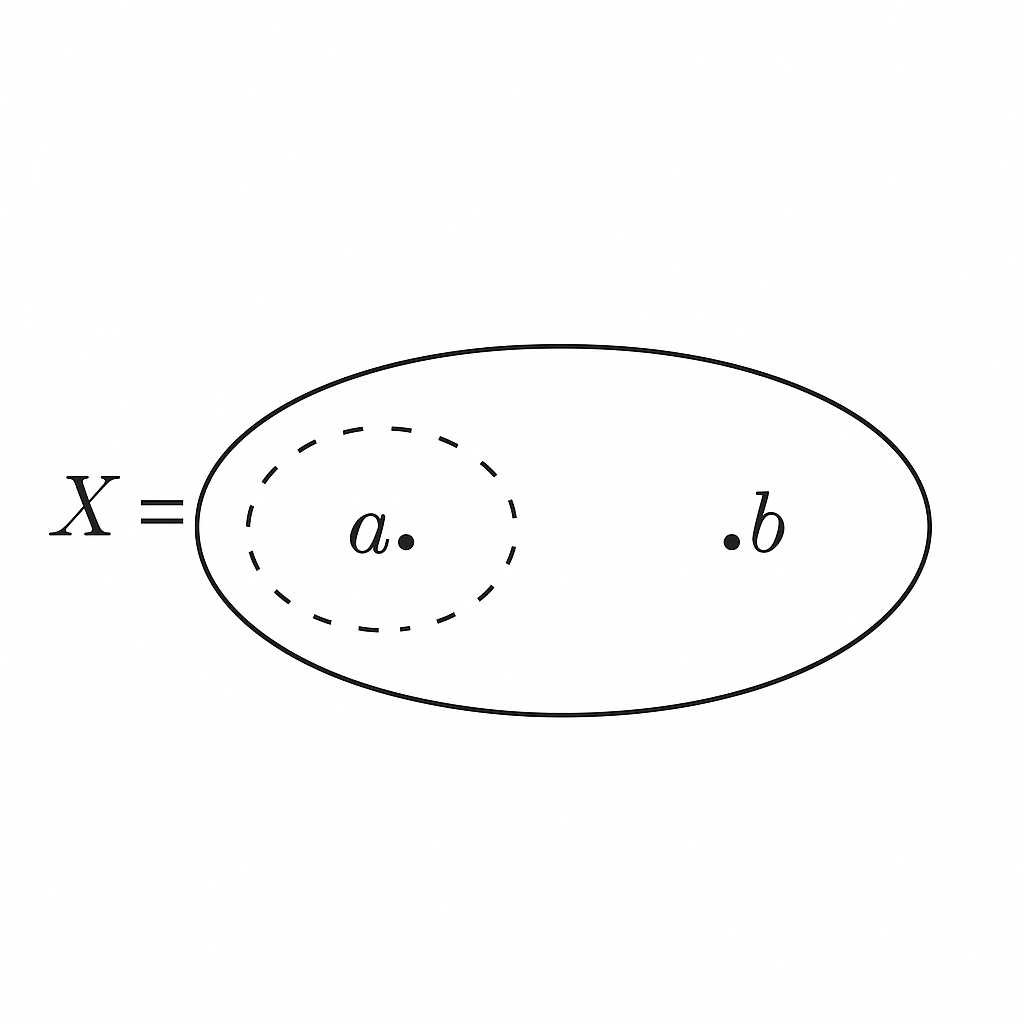
\includegraphics[width=0.5\textwidth]{graph/nonhausdorff.png}
        \caption{A non-Hausdorff space}
    \end{figure}    
\end{remark}
Hausdorff space is a nice axiom to ensure the separtion of points such that limit can be defined uniquely in the space, it is the topic we will discuss in other section, here we just see how hausdorff space interact with compact space:
\begin{proposition}
Let \(X \in \mathbf{Top}\)\\

(1) \(A\subset X\) is compact and \(X\) is Hausdorff, then \(A\) is closed.\\

(2) \(Y\) is a compact subspace of a Hausdorff space \(X\), then the subset of \(Y\) is compact if and only if it is closed in \(X\).\\

(3) \(f: X \to Y\) is a continous bijection, \(X\) is compact and \(Y\) is Hausdorff, then \(f\) is a homeomorphism.
\end{proposition}
\begin{proof}
    
\end{proof}

\begin{remark}
    (1) and (2) is the classic result in metric space, but generally it need the Hausdorff condition, otherwise it can fail, for example consider the non-Hausdorff space just now, the singleton \(\{b\}\) is compact but not closed.\\

    (3) is a very useful result to verify whether a continous bijection is a homeomorphism or not, for example in UPQ-TOPO, if we add that \(Y\) is Hausdorff, then \(\bar{f}\) is furthermore a homeomorphism if the quotient space is compact.
\end{remark}

As we mentioned just now, the finite intersection of compact sets is compact, but the countable intersection is not necessary compact, we can add some condition now:
\begin{proposition}[Nested sequence]$ \\$ \label{nestseq}
    Let \(X \in \mathbf{Top}\), and \(\{C_n\}_{n \in \nn}\) be a decreasing sequence of non-empty compact subsets of \(X\), then the intersection \(\bigcap_{n \in \nn} C_n\) is non-empty and compact.
    
\end{proposition}
\begin{proof}
\end{proof}

\begin{corollary}
Real number system is complete.
\end{corollary}
\begin{proof}
    
\end{proof}

\begin{remark}
    An famous example of nested sequence is the \textbf{Cantor set}, it is a typical fractal set with uncountbale points but zero measure, it can be constructed by removing the open middle third interval of \([0,1]\) recursively:
\[C=\bigcap_{n\geq 0}C_n\]
with \(C_0 :=[0,1]\) and \(C_n := \frac{C_{n-1}-1}{3} \cup (\frac{2}{3}+\frac{C_{n-1}}{3})\) for \(n\geq 1\). The figure below shows the construction:
\begin{figure}[H]
    \centering
    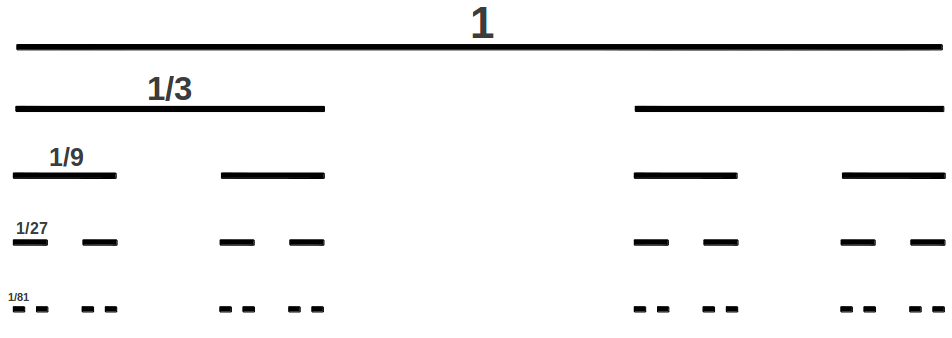
\includegraphics[width=0.8\textwidth]{graph/CantorSet.png}
    \caption{Construction of Cantor set}
\end{figure}
\end{remark}
Clearly, by the nested sequence proposition, the cantor set is non-empty and compact. It is zero measure by the monotone convergence of measure:
\[m(C) = m (\lim_{N} \bigcap_{n=0}^{N} C_n) = \lim_{N} m(C_N) = \lim_{N} \frac{2^N}{3^N} = 0\]
And the set is uncountbale, it is not so easy to prove, but roughly speaking,
\[C = \{x \in [0,1]| [x]_3 = 0.a_1a_2a_3... \text{ for some } a_i \in \{0,2\}\}
\]
every points in cantor set can be represented by a ternary decimal with only \(0\) and \(2\), and such a set is uncountable with cardinality \(2^{\aleph_0}\) (PLS see more details in measure theory).

\subsubsection*{Tychonoff's theorem*}
The last part of this section is to clarify the compactness of arbitrary product of compact spaces, it is a useful result in analysis (less so to geometry).\\

The first thing is to rigorous the deinition of product topological space, in the case of finite the definition is natrual, but in the case of infinite, we need to be careful. If we copy the definition of finite product, let \(\{X_i\}_{i \in I}\) be a family of topological spaces, then the topology on \(\prod_{i \in I}X_i\) is defined as
\[\mathcal{T}= \{\prod_{i \in I} U_i | U_i \text{ is open in } X_i\}\]
\begin{example}
    We consider the product space \(([0,1]^{\nn},\mathcal{T})\), we can prove that the space is not compact under above topology:

    Take an open cover \(\mathcal{O}=\{U_0,U_1,U_2,\ldots\}\) where 
    \[U_0 = \{(a_1,a_2,\dots)|a_i <\frac{1}{2}, \quad i\geq 1\}\]
    and for any \(k \geq 1\),
    \[U_k = \{(a_1,a_2,\dots)|a_k > \frac{1}{4}\}\]
    We notice that if we want to choose a subcover from \(\mathcal{O}\), then \(U_0\) must be chosen, otherwise the point \((0,0,0,\dots)\) can not be covered.\\

    Suppose that we have chosen a finite subcover \(\{U_0,U_{a_1},...,U_{a_l}\}\) then we can take some \(k \notin \{a_1,...,a_l\}\), then we construct a point \(a\) with \(a_k=1\) and other coordinates equal to \(0\), then the point \(a\) can not be covered by the finite subcover, so we finish the proof.
\end{example}
It shows that the above topology is too fine to ensure the compactness of product space, so we need to modify the definition of product topology. The universal properties of product space can help us to choose the right topology, for any product set \(\prod_{i \in I} X_i\) we have a natural projection map
\[\pi_k:\prod_{i \in I}X_i \to X_k, \quad (x_i)_{i \in I} \mapsto x_k\]
In languae of category, we expect the projection will be a morphism in \(\mathbf{Top}\), that means the projection should be continous, hence the topology on the product set should be at least fine as the pullback topology induced by \(\pi_k\):
\[\mathcal{T}_k:= \{\pi_k^{-1}(U)|U \text{ is open in } X_k\}\]
In detail, \(\pi_k^{-1}(U)\) =  \(\prod_{i \in I}Y_i\) With
\[Y_k=U,\quad Y_i=X_i \text{ for } i \neq k\]
And we expect all i-projections are continous, so the smallest topology will be generated by choosing \(\bigcup_{i \in I}\mathcal{T}_i\) as the basis for topology, so we can get a more rough topology than before, and we conclude them by a foraml definition:
\begin{definition}
    Let \((X_i,\mathcal{T}_i) \in \mathbf{Top}\), and \(i \in I\) a non-empty index set.\\
    
    -The product topology on the product set \(\prod_{i \in I}X_i\) is defined by
    \[\mathcal{B}:= \{\prod_{i \in J} U_i \times \prod_{i \in I \setminus J} X_i | J \subseteq I \text{ finite}, U_i \in \mathcal{T}_i\}\]

    - The box topology on the product set is defined by
    \[\mathcal{B}_{box} := \{\prod_{i \in I}U_i| U_i \in \mathcal{T}_i\}\]
\end{definition}
Just remind that the product topology is rougher than box topology, and it is the smallest topology sucht that all projections are continous maps. The above example shows that the box topology can not keep the compactness of product space. \textbf{In particualr, the product topology is equal to box topology when the product is finite.}\\

Another thing needed is an equivalent statement of compactness.
\begin{definitionplain*}
    A collection of subsets \(\{C_i\}_{i \in I}\) in a topological space \(X\) is said to have the \textbf{FIP(finite intersection property)} if for any finite subset \(J \subset I\), \(\bigcap_{j \in J} C_j \neq \emptyset\).
\end{definitionplain*}

In a short word, \(FIP\) means that any finite intersection of subcollection is nonn-empty.
\begin{proposition}[FIP-COMPACT]$ \\$
    Let \(X \in \mathbf{Top}\), then \(X\) is compact if and only if for any collection of closed subsets \(\{C_i\}_{i \in I}\) with properties FIP, the intersection \(\bigcap_{i \in I} C_i\) is non-empty.
\end{proposition}
\begin{proof}
    
\end{proof}
\begin{remark}
    A direct corollary is the nested sequence propostion \ref{nestseq}, because a decreasing sequence of non-empty closed subsets obviously has the property FIP.
\end{remark}

\begin{theorem}
    [Tychonoff's theorem] $ \\$
    Let \(\{X_i\}_{i \in I}\) be a family of compact spaces, then the product space \(\prod_{i \in I} X_i\) with product topology is also compact.
\end{theorem}

\subsection{Topological axioms}
The topology determines the structure of the space, if we have a topological space we can naturally study its structure by the open sets. Conversely, if we want to construct a topological space, we need to define a topology by choosing some open sets, usually it is difficult to write all open sets down directly, we need a collection like "base" for vector space.

\begin{definition}
    Let \(X\) be a non-empty set, a collection \(\mathcal{B} \subset \mathcal{P}(X)\) is called \textbf{a basis for a topology} on \(X\) if\\

    (1) For any \(x \in X\), there is at least one basis element \(B \in \mathcal{B}\) such that \(x \in B\).\\
    (equivalently, \(\bigcup_{B \in \mathcal{B}} B = X\))\\

    (2) If \(x\) belongs to the intersection of two basis elements \(B_1,B_2 \in \mathcal{B}\), then there is a basis element \(B_3 \in \mathcal{B}\) such that \(x \in B_3 \subseteq B_1 \cap B_2\).\\
    (equivalently, finite intersection of basis elements is in the basis.)\\

    The topology \(\mathcal{T}\) generated by \(\mathcal{B}\) is defined as
    \[\mathcal{T} := \{U \subset X | \forall x \in U, \exists B \in \mathcal{B} \text{ such that } x \in B \subseteq U\}\]
    i.e. the open set is of the form of union of basis elements.
\end{definition}

We need to verify that the axiom of topology generated by basis:

(1) \(X \in \mathcal{T}\) since by (1) of basis definition, we can find a basic open sets \(B_x \in \mathcal{B}\) for any \(x\), then 
\[X = \bigcup_{x \in X}B_x\] satisfy the definition of open sets. For empty-set, it holds formally by 
\[ \emptyset  = \bigcup_{x \in \emptyset }B_x\]
Howerver, no points in empty-set implies that the condition is vacuously true, so \(\emptyset \in \mathcal{T}\).

(2) For any \(U,V \in \mathcal{T}\), and any \(x \in U \cap V\), by the definition of open sets, there are basis elements \(B_1,B_2 \in \mathcal{B}\) such that
\[x \in B_1 \subseteq U \quad \text{and} \quad x \in B_2 \subseteq V\]
Then \(B_1 \cap B_2\) is a basis element containing \(x\) and is contained in \(U \cap V\), thus \(U \cap V \in \mathcal{T}\).

(3) For any collection of open sets \(\{U_i\}_{i \in I} \subset \mathcal{T}\), and any \(x \in \bigcup_{i \in I} U_i\), then there is some \(j \in I\) such that \(x \in U_j\), by the definition of open sets, there is a basis element \(B \in \mathcal{B}\) such that
\[x \in B \subseteq U_j \subseteq \bigcup_{i \in I} U_i\]
thus \(\bigcup_{i \in I} U_i \in \mathcal{T}\).\\

A typical example of basis is the standard basis of \(\rr\):
\[\mathcal{B} = \{(a,b) \mid a<b, a \text{ and } b \in \qq\}\]
It is easy to verify that \(\mathcal{B}\) satisfies the two conditions of basis, and the topology generated by \(\mathcal{B}\) is the standard topology on \(\rr\). Generally, any \textbf{metric space} \((X,d)\) has a topology base which generates the metric topology:
\[\mathcal{B} = \{B(x,r) | x \in X, r >0\}\]
where \(B(x,r) = \{y \in X | d(x,y) < r\}\) is the open ball with center \(x\) and radius \(r\), hence sometimes we \textbf{call open ball as basic open set} in metric space.

\subsection*{Countable axiom}
In analysis, we always use the tool of sequences: we take a voisinage of a point, then choose another point in the voisinage, and repeat this process to the smaller voisinage, and so on, finally we get a sequence \(\{a_n\}_{n \in \nn}\) which converges to the point and a sequence of voisinage \(\{V_n\}_{n \in \nn}\), they are all countable! Hence, at least the topology of the space allows us to choose countable open sets, that is the \textbf{motivation} of countable axiom in topology.

\begin{definition}
    Let \((X,\mathcal{T}) \in \mathbf{Top}\) be a topological space,\\

    (1) \(X\) is called \textbf{first-countable} if for any point \(x \in X\), there is a countable (local) basis \(\mathcal{B}_x = \{B_{x,n}\}_{n \in \nn}\) of open sets such that for any open set \(U\) containing \(x\), there is some \(B_{x,n} \in \mathcal{B}_x\) such that
    \[x \in B_{x,n} \subseteq U\]
    (i.e. each point has a countable local basis).\\

    (2) \(X\) is called \textbf{second-countable} if there exists a countable basis for topology \(\mathcal{T}\).
\end{definition}

Clearly, second-countable implies first-countable, because for any \(x \in X\), we can just choose the local basis \(\mathcal{B}_x = \mathcal{B}\). Conversely, first-countable does not imply second-countable, for example consider the discrete topology on \(\rr\)
\[\mathcal{T}_d = \mathcal{P}(\rr)\]
it is first-countable since we can choose \(\mathcal{B}_x = \{\{x\}\}\) for any \(x \in \rr\), but it is not second-countable since the smallest open set containing \(x\) is \(\{x\}\) itself, so at least
\[ \{\{x\} \mid x \in \rr\} \subset \mathcal{B}\]
which implies that \(\mathcal{B}\) is uncountable.\\

Another example is \textbf{cofinite topology} on \(\rr\)
\[\mathcal{T}_c = \{U \subset X \mid \#X\setminus U<+\infty\} \cup \{\emptyset,\rr\}\]
We can prove that it is neither first-countable nor second-countable (\textbf{Verify!}).\\

In a short word, countable axiom determine \textbf{whether we can study convergence using sequences} (instead of the more general notions of nets or filters). Second-countable axiom can implies other nice type of space as following:
\begin{proposition}
    Let \(X \in \mathbf{Top}\) be a second-countable space, then\\

    (1) \(X\) is \textbf{separable}, i.e. there is a countable dense subset \(D \subset X\).\\

    (2) \(X\) is \textbf{Lindelöf}, i.e. every open cover of \(X\) has a countable subcover.
\end{proposition}
\begin{proof}
    (1) Since \(X\) is second-countable, we can find a countable basis \(\mathcal{B}\) for the topology \(\mathcal{T}\). For each \(B \in \mathcal{B}\), we can find a point \(x_B \in B\). Then the set \(D = \{x_B \mid B \in \mathcal{B}\}\) is countable and dense in \(X\).

    (2) Let \(\{U_i\}_{i \in I}\) be an open cover of \(X\). For each \(x \in X\), we can find a basis element \(B_x \in \mathcal{B}\) such that \(x \in B_x \subseteq U_i\) for some \(i \in I\). Since \(\mathcal{B}\) is countable, we can extract a countable subcover \(\{U_{i_n}\}_{n \in \nn}\) that covers \(X\).
\end{proof}
A nice equivalence can be concluded in mertic space:
\begin{corollary}
    In metric space
    \[\text{second-countable} \iff \text{separble} \iff \text{Lindelöf}\]
\end{corollary}
\begin{proof}
    outline:\\
    (a) Lindelöf \(\implies\) separable in metric space\\
    We consider the n-open cover
    \[\mathcal{U}_n = \{B(x,1/n) \mid x \in X\}\]
    By Lindelöf property, each n-open cover has a countable subcover
    \[\mathcal{V}_n=\{B(x_{n,k},1/n) \mid k\in \nn\}\]
    then we can choose a subset of \(X\) as
    \[D = \{x_{n,k} \mid  n,k \in \nn\}\]
    then we can prove that \(D\) is dense in \(X\).\\
    (b) separable \(\implies\) second-countable in metric space\\
    It is simlar to find a countable basis for topology in \(\rr\) using the dense subset \(\qq\). Suppose \(D\) is a countable dense subset of \(X\), then we can choose
    \[\mathcal{B} = \{B(d,q) \mid d\in D,q \in \qq\}\]
    then we can prove it is a basis for topology, and verify the topology generated by \(\mathcal{B}\) is same as the metric topology.\\
    (c) conclude by the above proposition.
\end{proof}

\subsection*{Separtion Axiom}
The motivation of separation axiom is to ensure the separation of points or sets using open sets, it is useful to define limit and continuity in topology. We can define the sequence of limit in topology instead of \(\epsilon-\delta\) language as following:
\begin{definitionplain*}
    Let \((X,\mathcal{T}) \in \mathbf{Top}\) be a topological space, and \(\{x_n\}_{n \in \nn}\) be a sequence in \(X\), a point \(x \in X\) is called a \textbf{limit} of the sequence (or \textbf{converges} to \(x\)) if for any open set \(U\) containing \(x\), there is some \(N \in \nn\) such that for any \(n \geq N\), \(x_n \in U\).
\end{definitionplain*}
We can construct an example such that a sequence has different limits:
\[X = \{0,1,2\}, \quad \mathcal{T} = \{\emptyset,X,\{2\},\{1,2\}\}\]
In this case, we consider the constant sequence \(x_n = 2\), then we can find that both \(1\) and \(2\) are limits of the sequence \textbf{(checking the definition!)}. Hence it is necessary to clasisfy the space to aviod the case like this.

Another motivation is from the view of outer measure. We want to define the measure of a set \(A\) by the infimum of the measures of open sets containing \(A\):
\[m^*(A) = \inf\{m(U) | U \supset A, U \text{ is open}\}\]
where \(m\) is a measure defined on basic open sets. Now if \(A=A_1 \cup A_2\) a disjoint union of two sets, and we hope that
\[m^*(A) = m^*(A_1)+m^*(A_2)\]
then clearly here we must allow the existence of two disjoint open sets \(U_1,U_2\) such that \(A_1 \subset U_1\) and \(A_2 \subset U_2\), otherwise the equality can fail, the correspondece to this requirement is the normal space in topology.\\

\begin{definition}
    Let \((X,\mathcal{T}) \in \mathbf{Top}\) be a topological space,\\

    (1) \(X\) is called a \textbf{T0 space} if for any two different points \(x,y \in X\), there is an open set \(U \in \mathcal{T}\) such that
    \[x \in U, y \notin U \quad \text{or} \quad y \in U, x \notin U\]

    (2) \(X\) is called a \textbf{T1 space} if for any two different points \(x,y \in X\), there are two open sets \(U,V \in \mathcal{T}\) such that
    \[x \in U, y \notin U\quad \text{and} \quad y \in V, x \notin V\]

    (3) \(X\) is called a \textbf{Hausdorff space (T2 space)} if for any two different points \(x,y \in X\), there are two open sets \(U,V \in \mathcal{T}\) such that
    \[x \in U, y \in V, U \cap V = \emptyset\]

    (4) \(X\) is called a \textbf{regular space (T3 space)} if it is a \(T1\) space such that for any closed set \(C \subset X\) and any point \(x \notin C\), there are two open sets \(U,V \in \mathcal{T}\) such that
    \[x \in U, C \subset V, U \cap V = \emptyset\]

    (5) \(X\) is called a \textbf{normal space (T4 space)} if it is a \(T1\) space such that for any two disjoint closed sets \(C_1,C_2 \subset X\), there are two open sets \(U,V \in \mathcal{T}\) such that
    \[C_1 \subset U, C_2 \subset V, U \cap V = \emptyset\]
\end{definition}
\begin{remark}
    (1) In above definition, we have a good chain of implications:
    \[T4 \implies T3 \implies T2 \implies T1 \implies T0\]
    it reflects the strenghth of separation axiom.

    (2) In above definition, The condition of \(T1\) space in \(T3\) and \(T4\) can not be omitted (even if it satisfies automatically in many cases), otherwise we can not get above implications, for example consider a trival non-Hausdorff space 
    \[X=\{a,b\}, \quad \mathcal{T} = \{\emptyset, X\}\]
    but we notice that it is normal space since the unique closed sets are \(\emptyset\) and \(X\), and trivially we can find two disjoint open sets containing them \textbf{(it is just a stupid logical game)}, i.e. \(\emptyset\) and \(X\).

    (3) The most used separation axiom is Hausdorff space, because it is easy to verify and have many good properties. \textbf{An equivalent statement} of Hausdorff space is that the diagonal set \[\Delta = \{(x,x) | x \in X\} \subset X \times X\] is closed in the product space \(X \times X\) \textbf{(verify!)}.

    (4) Any \textbf{metric space} is normal space, so it is also \(T3,T2,T1,T0\) space.
\end{remark}

It is not free to get a space with strong separtion, we can add some condition such that we can get a nice space:
\begin{proposition}
    Let \(X \in \mathbf{Top}\) be a topological space, then\\

    -   If \(X\) is \(T3\) and second-countable, then \(X\) is \(T4\).\\

    -   If \(X\) is \(T2\) and compact, then \(X\) is \(T4\).
\end{proposition}
\begin{proof}
see Munkres' Topology book \textbf{(section 32)}.    
\end{proof}
It is important to see the stability of separation axiom under different operations, it is easy to verify.

\begin{proposition}
    The stability of separtion axiom:\\

    (1-subspace) any subspace of a \(T_i\) space is still a \(T_i\) space for \(i=0,1,2,3\).\\

    (2-finite product) the finite product of \(T_i\) spaces is still a \(T_i\) space for \(i=0,1,2,3\).\\

    (3-product) The any product of \(T_i\) spaces is still a \(T_i\) space for \(i=0,1,2\).\\


    (3-map) Let \(f:X \to Y\) be a continuous bijection and \(Y\) is a \(T_i\) space for \(i=0,1,2,3,4\), then \(X\) is still a \(T_i\) space.
\end{proposition}
\begin{proof}
    Just some verification\dots
\end{proof}

\begin{remark}
    (1) Normal space is not stable in above proposition, an counterexample is \textbf{Tychonoff plank}.\\

    (2) The product of two normal spaces may not be normal, an counterexample is \textbf{Sorgenfrey plane}. We consider the Sorgenfrey line (lower limit topology) \(\rr_l\) generated by basis
    \[\mathcal{B} = \{[a,b) | a < b\}\]
    It is normal becasue the topology is finer than standard topology:
    \[(a,b) = \bigcup_{x \in (a,b)}[x,b)\]
    but the product space \(\rr^2_l\) is not normal.

    (3) Many examples can be found in 拓扑空间与线性拓扑空间中的反例 by 汪林.

    (4) the separation can not be tranistive like compacteness and connectedness, i.e. \(f(X)\) may not be \(T_i\) space even if \(X\) is \(T_i\) space. It is reasonable since continous map implies that the the topology of \(X\) is finer than the pullback topology induced by \(f\), it gives no information about the topology of image space.
\end{remark}

Finally, we will conclude some classic result in analysis, and we will see that how separation axiom works in them: In metric spaces\\

(1) a sequence has at most one limit.\\

(2) \(x \in \overline{A}\) iff there is a sequence \(\{a_n\}_{n \in \nn}\) of A such that \(a_n\) converges to \(x\).\\

(3) A function \(f:X \to Y\) is continuous iff for any sequence \(\{x_n\}_{n \in \nn}\) converging to \(x\), the sequence \(\{f(x_n)\}_{n \in \nn}\) converges to \(f(x)\).\\

In general, (1) holds if \(X\) is \textbf{Hausdorff space}, (2) and (3) hold if \(X\) is \textbf{first-countable} space.


\newpage

\subsection{Topological group}

Group and Topological space is two different objects, group is algebraic structure, topological space is geometric structure, but it is not strange to combine them together.

\begin{definition}
A \textbf{topological group} is a object \((G,\mathcal{T},\cdot)\) such that
\begin{itemize}
    \item \((G,\cdot)\) is a group
    \item \((G,\mathcal{T})\) is a topological space
    \item The group structure is compatible with topological structure, i.e. multiplication 
    \[m: G \times G \to G, \quad (x,y) \mapsto x \cdot y\]
    and inverse \[i: G \to G, \quad x \mapsto x^{-1}\]
    are continuous maps.
\end{itemize} 
\end{definition}

Let us see some examples of topological groups
\begin{example}
    \item (1) \(\rr^n\) with addition and standard topology is a topological group.
    \item (2) \(\sph^1 = \{z \in \cc | |z|=1\}\) with multiplication and subspace topology of \(\cc\) is a topological group. 
    \item (3) The torus \(T\) can be seen as the product of two topological groups \(\sph^1 \times \sph^1\), by the universal property of product topology, \(T\) is also a topological group.
    \item (4) Any discrete group with discrete topology is a topological group.
    \item (5) \(GL(n,\rr)\) with multiplication and subspace topology of \(\rr^{n^2}\) is a topological group.
\end{example}


we first prove some properties of topological group, the results are not diffcult, but it is always useful.

\begin{proposition}
    Let \(G\) be a topological group and \(H\) be a subgroup of \(G\), then\\

    (1-translation) For any \(g \in G\), the left-translation \(L_g: G \to G, x \mapsto g \cdot x\) and right-translation \(R_g: G \to G, x \mapsto x \cdot g\) are homeomorphisms.\\

     (2-open) If \(H\) is open, then \(H\) is closed and \(G/H\) is discrete.\\

    (3-Hausdorff)
    \[
    \begin{aligned}
    G &\text{ is Hausdorff} &&\Longleftrightarrow\ \{e\}\text{ is closed}.\\
    G/H &\text{ is Hausdorff} &&\Longleftrightarrow\ H\text{ is closed in }G.
    \end{aligned}
    \]

    (4-homogeneous) If \(G\) is connect, then any voisinage of \(\{e\}\) can generate the group.\\

    (5-CC) Let \(G_0\) be the connected component of \(G\) containing \(e\), then \(G_0\) is a closed normal subgroup of \(G\), and any connected component of \(G\) is homeomorphic to \(G_0\).

\end{proposition}

\begin{proof}
    
\end{proof}

\begin{remark}
    Translation is very important in topological group, group is a object with symmetry and translation is a way to keep symmetry. For example, let \(x,y\) be two different points in \(G\), then the translation \(L_{yx^{-1}}\) is a homeomorphisms which maps \(x\) to \(y\), therefore each point of \(G\) share the same topological stucture, so the local property is same as golbal poerperty, that means topological group is a \textbf{homogeneous space}.
\end{remark}

the fundamental theorem of group homeomorphisms can be extended to topological group, in the discussion of topological group, we hope the map between two objects can preserve both two structures, that means the map is both a morphism of group and a continous map. 

\begin{example}
    We consider two topological groups: the first is \(\rr\) with addition and standard topology, the second is \(\sph^1\) with multiplication and subspace topology of \(\cc\) (or \(\rr^2\)). We define a map 
    \[
    \varphi: \rr \to \sph^1, \quad x \mapsto e^{2\pi i x}.
    \]
    (1) \(\varphi\) is a surjective group morphism with \(\ker \varphi = \mathbb{Z}\).\\
    (2) By UPQ-GRP, there is a unique group isomorphism \(\bar{\varphi}: \rr/\mathbb{Z} \to \sph^1\) such that \[\rr/\zz \cong \sph^1 \]
    (3) By UPQ-TOPO, \(\bar{\varphi}\) is also a continous bijection since \(\varphi\) is continous.\\
    (4) Notice that \(\sph^1\) is a Hausdorff space, \(\rr/\zz\) is compact (verify!) so \(\bar{\varphi}\) is automatically a homeomorphism.
\end{example}
We define the \textbf{isomorphism} between two topological groups are an application which is both \textbf{a group isomorphism} and \textbf{a homeomorphism}, the above examples shows that \(\rr/\zz\) and \(\sph^1\) are isomorphic as topological groups, with the similar techniques we can prove that \(SO(2)\) is also isomorphic to \(\sph^1\) as a topological group. We can generalized the result to be a so-called universal properties:
\begin{theorem}
    [UPQ-TGRP] $ \\$
    Let \(G\) and \(K\) be two topological groups, and \(\varphi: G \to K\) be a topological group morphism (i.e. continuous morphism of group), then there is a unique continous morphism of groups \(\bar{\varphi}: G/H \to K\) such that the digaram commutes
    % https://q.uiver.app/#q=WzAsMyxbMCwwLCJHIl0sWzIsMCwiSyJdLFswLDIsIkcvXFxrZXIgXFx2YXJwaGkiXSxbMCwyLCJcXHBpIiwyLHsic3R5bGUiOnsiaGVhZCI6eyJuYW1lIjoiZXBpIn19fV0sWzAsMSwiXFx2YXJwaGkiXSxbMiwxLCJcXGV4aXN0ISBcXGJhcntcXHZhcnBoaX0iLDIseyJzdHlsZSI6eyJib2R5Ijp7Im5hbWUiOiJkYXNoZWQifX19XV0=
\[\begin{tikzcd}
    G && K \\
    \\
    {G/\ker \varphi}
    \arrow["\varphi", from=1-1, to=1-3]
    \arrow["\pi"', two heads, from=1-1, to=3-1]
    \arrow["{\exists! \bar{\varphi}}"', dashed, from=3-1, to=1-3]
\end{tikzcd}\]
furthermore, if  the following conditions hold:\\
(1) \(\varphi\) is surjective,\\
(2) \(K\) is Hausdorff,\\
(3) \(G/\ker \varphi\) is compact,\\
then \(\bar{\varphi}\) is an isomorphism of topological groups.
\end{theorem}

\newpage
\section{Dual space and category}

In this section, we will the structure of dual in the view of category, and then discuss some properties of dual space.

\begin{definition}
    Let \(V\) be a vector space over a field \(K\). The \textbf{dual space} of \(V\), denoted \(V^*\), is the set of all linear functionals from \(V\) to \(K\):
    \[
    V^* = \mathcal{L}(V, K) = \{ f: V \to K \mid f \text{ is linear} \}.
    \]
\end{definition}

\begin{proposition} \label{dualvectorspace}
    The dual space \(V^*\) is a vector space over \(K\) with the following operations:
    \begin{itemize}
        \item (Addition) If \(f, g \in V^*\), then \((f + g)(v) = f(v) + g(v)\) for all \(v \in V\).
        \item (Scalar multiplication) If \(f \in V^*\) and \(\alpha \in K\), then \((\alpha f)(v) = \alpha f(v)\) for all \(v \in V\).
    \end{itemize}
\end{proposition}

    The dual space \(V^*\) captures the notion of linear functionals on \(V\) and provides a way to study the properties of \(V\) through its dual. Another important concept related to dual space is the dual map induced by a linear map

\begin{proposition} \label{dualmap}
    Let \(T: V \to W\) be a linear map between vector spaces \(V\) and \(W\). The \textbf{dual map} \(T^*: W^* \to V^*\) is defined by
    \[
    T^*(g) = g \circ T
    \]
    for all \(g \in W^*\), it is a linear map induced by \(T\).\\
    Furthermore, \(T^*\) satisfies the following properties:
    \begin{itemize}
        \item (Preservation of identity) for any identity linear map \(I:V^* \to V^*\), \(I^*\) is the identity linear map on \(V^*\).
        \item (Preservation of composition) for any linear maps \(T: V \to W\) and \(S: W \to U\), we have \((S \circ T)^* = T^* \circ S^*\).
    \end{itemize}
\end{proposition}


    \begin{proof}
        To show that \(T^*\) is linear, we need to verify that it preserves addition and scalar multiplication. Let \(g_1, g_2 \in W^*\) and \(\alpha \in K\). Then, for any \(v \in V\):
        \[
        T^*(g_1 + g_2)(v) = (g_1 + g_2)(T(v)) = g_1(T(v)) + g_2(T(v)) = T^*(g_1)(v) + T^*(g_2)(v).
        \]
        Thus, \(T^*(g_1 + g_2) = T^*(g_1) + T^*(g_2)\).

        Next, for scalar multiplication:
        \[
        T^*(\alpha g)(v) = (\alpha g)(T(v)) = \alpha g(T(v)) = \alpha T^*(g)(v).
        \]
        Therefore, \(T^*(\alpha g) = \alpha T^*(g)\).

        Since \(T^*\) preserves both addition and scalar multiplication, it is a linear map.
        Now, we verify the preservation of identity. Let \(I: V \to V\) be the identity map. For any \(g \in V^*\) and \(v \in V\):
        \[I^*(g)(v) = g(I(v)) = g(v).\]
        Thus, \(I^*(g) = g\), which shows that \(I^*\) is the identity map on \(V^*\).

        Finally, we verify the preservation of composition. Let \(T: V \to W\) and \(S: W \to U\) be linear maps. For any \(h \in U^*\) 
        \[
        (S \circ T)^*(h) = h\circ(S \circ T)   = (h \circ S)\circ T = T^*(S^*(h))=(T^* \circ S^*)(h).
        \]
    \end{proof}

After knowing the basic definition of dual space and dual map, we can conclude like following:
\begin{itemize}
    \item We try to see dual as some function, which maps a vector space to the dual space (by proposition \ref{dualvectorspace}), so we naturally define \(\mathbf{Vect}_K\) to be the set of all vector spaces over field \(K\), then dual can be seen as a function in it
    \[(-)^*:\mathbf{Vect}_K \to \mathbf{Vect}_K, \quad V \mapsto V^*\]
    that means dual can be seen \textbf{as a function between classes} (In the set theory, the set of sets is called classes).

    \item Furthermore, dual is not only a function between classes, each linear map \(T: V \to W\) induces a dual map \(T^*: W^* \to V^*\) (by proposition \ref{dualmap}), so we can get annother information about dual: it can be seen as \textbf{a function between sets of morphisms} (in the vector spaces, a morphism is a linear map, which preserves the vector space structure), hence we can define dual as following:
    \[( - )^* : \mathcal{L}(V,W) \to \mathcal{L}(W^*, V^*), \quad T \mapsto T^*\]
\end{itemize}

That is two level of dual, and we can draw a picture like following:
% https://q.uiver.app/#q=WzAsNCxbMCwwLCJWIl0sWzIsMCwiVyJdLFswLDIsIlZeKiJdLFsyLDIsIldeKiJdLFswLDIsIigtKV4qIiwxLHsic3R5bGUiOnsiYm9keSI6eyJuYW1lIjoiZGFzaGVkIn19fV0sWzAsMSwiVCJdLFsxLDMsIigtKV4qIiwxLHsic3R5bGUiOnsiYm9keSI6eyJuYW1lIjoiZGFzaGVkIn19fV0sWzMsMiwiVF4qIl0sWzUsNywiKC0pXioiLDEseyJzaG9ydGVuIjp7InNvdXJjZSI6MjAsInRhcmdldCI6MjB9LCJzdHlsZSI6eyJib2R5Ijp7Im5hbWUiOiJkYXNoZWQifX19XV0=
\[\begin{tikzcd}
	V && W \\
	\\
	{V^*} && {W^*}
    \arrow[""{name=0, anchor=center, inner sep=0}, "T", from=1-1, to=1-3]
    \arrow["{(-)^*}"{description}, dashed, from=1-1, to=3-1]
    \arrow["{(-)^*}"{description}, dashed, from=1-3, to=3-3]
    \arrow[""{name=1, anchor=center, inner sep=0}, "{T^*}", from=3-3, to=3-1]
    \arrow["{(-)^*}"{description}, Rightarrow, dashed, from=0, to=1]
\end{tikzcd}\]
We should pay attention to the level of dual, the first level is the function between classes, the second level is the function between sets of morphisms, we have the first level, and then we can get the second level by naturally definition, that is why category is a powerful tool! In set theory, we only have elements in a set, and then we use functions to connect two sets, but now we hope to construct a class contatining sets, and then use a function to connect two classes, but that is not ennough, we also need to connect a morphism of two sets in a class to another morphism of two sets in another class, that is the second level of function.


\begin{definition}[Category]
A category $\mathcal{C}$ consists of the following data:
\begin{itemize}
  \item a unique class of \textbf{objects}(sets or any other mathematical objects)
        \[
        \Ob(\mathcal{C});
        \]
  \item for every pair of objects $A, B \in \Ob(\mathcal{C})$, a set of morphisms
        \[
        \Hom_{\mathcal{C}}(A,B);
        \]
  \item for every triple of objects $A, B, C \in \Ob(\mathcal{C})$, a function called \textbf{composition}
        \[
        \circ : \Hom_{\mathcal{C}}(B,C) \times \Hom_{\mathcal{C}}(A,B)
        \longrightarrow \Hom_{\mathcal{C}}(A,C),
        \quad (g,f) \mapsto g \circ f;
        \]
  \item for each object $A \in \Ob(\mathcal{C})$, there exists an \textbf{identity morphism}
        \[
        \mathrm{id}_A \in \Hom_{\mathcal{C}}(A,A).
        \]
\end{itemize}
These data satisfy the following axioms:

  \item \textbf{Associativity:}
        for all \(f\in \Hom_{\mathcal{C}}(A,B)\), \(g\in \Hom_{\mathcal{C}}(B,C)\), and \(h\in \Hom_{\mathcal{C}}(C,D)\):
        \[
        h \circ (g \circ f) = (h \circ g) \circ f.
        \]
  \item \textbf{Identity:}
        for all \(f\in \Hom_{\mathcal{C}}(A,B)\),
        \[
        f \circ \mathrm{id}_A = f = \mathrm{id}_B \circ f.
        \]

\end{definition}

\begin{remark}
    we often write the following to simplify the notation:
    \[A \in \mathcal{C} \iff A \in \Ob(\mathcal{C})\]
    and
    \[f:A \to B \iff f \in \Hom_{\mathcal{C}}(A,B)\]
    In set theory, we often see element as a point, similarly, in category theory, we often see object as a point, and morphism as an arrow between two points, so the category can be draw as a graph like following:
    % https://q.uiver.app/#q=WzAsNCxbMCwwLCJBIl0sWzAsMiwiQyJdLFszLDIsIkQiXSxbMiwwLCJCIl0sWzAsMCwiMV9BIl0sWzEsMSwiMV9DIiwyLHsicmFkaXVzIjotM31dLFsyLDIsIjFfRCIsMix7InJhZGl1cyI6LTN9XSxbMywzLCIxX0IiXSxbMCwzLCJmIiwxXSxbMywxLCJnIiwxXSxbMCwxLCJnXFxjaXJjIGYiLDFdXQ==
\[\begin{tikzcd}
	A && B \\
	\\
	C &&& D
	\arrow["{1_A}", from=1-1, to=1-1, loop, in=55, out=125, distance=10mm]
	\arrow["f"{description}, from=1-1, to=1-3]
	\arrow["{g\circ f}"{description}, from=1-1, to=3-1]
	\arrow["{1_B}", from=1-3, to=1-3, loop, in=55, out=125, distance=10mm]
	\arrow["g"{description}, from=1-3, to=3-1]
	\arrow["{1_C}"', from=3-1, to=3-1, loop, in=305, out=235, distance=10mm]
	\arrow["{1_D}"', from=3-4, to=3-4, loop, in=305, out=235, distance=10mm]
\end{tikzcd}\]
In the category we defined above, we only have four objects so by definition we at least have four identity morphisms (arrows start and end at the same point); and we only define two morphisms between different objects, i.e. \(f:A \to B\) and \(g:B\to C\), by composition we can get another morphism \(g \circ f: A \to C\), so actually we have six morphism in this category.
\end{remark}

Category is a strong concept to generalized the objects in mathematics.
\begin{example}
    \item (1) The category of sets: \[
\mathbf{Set} \;\Big|\;
\begin{array}{l}
  \text{object: all sets} \\
  \text{morphisms: functions between sets}
\end{array}
\]
Here a famous paradox in set theory is \textbf{Russell's paradox}, that shows that there does not exists a set containing all sets, otherwise a contradiction will arise according to the axiom of set theory. To avoid the paradox, we use classes instead of sets to define category, but that is not enough, because sometimes we hope to talk about the category of all categories, so a strong axiom called \textbf{Grothendieck universes} is needed here.

(2) The caetgory of groups:
\[
\mathbf{Grp} \;\Big|\;
\begin{array}{l}
  \text{object: all groups} \\
  \text{morphisms: group homomorphisms}
\end{array}
\]
(3) The category of topological spaces:
\[\mathbf{Top} \;\Big|\;
\begin{array}{l}
  \text{object: all topological spaces} \\
  \text{morphisms: continuous maps}
\end{array}
\]
(4) The category of vector spaces over a field \(K\):
\[
\mathbf{Vect}_K \;\Big|\;
\begin{array}{l}
  \text{object: all vector spaces over } K \\
  \text{morphisms: linear maps}
\end{array}
\]
\end{example}

In category, we usually ignore the elements of an object, and only care about the morphisms between two objects, so we will care about whether the morphism is injective, surjective or bijective. However, in the traditional definition of functions, the statment will depend on the elements of the set, so a lemma will be need here to generalized the definition of injection and so on in category.
\begin{lemma}
    Let \(f:A \to B\) be a function between two sets, then\\

    (1) \(f\) is injective if and only if for any set \(X\) and any two functions \(g_1,g_2: X \to A\), the left-cancellation holds: \[f \circ g_1 = f \circ g_2 \Rightarrow g_1 = g_2\] 

    (2) \(f\) is surjective if and only if for any set \(X\) and any two functions \(h_1,h_2: B \to X\), the right-cancellation holds:
    \[ h_1 \circ f = h_2 \circ f \Rightarrow h_1 = h_2\]
\end{lemma}

That will be very useful in the proof referring to universal properties. Another special morphism in a category is isomorphism, the definition is naturally same in group, vector space and so on.
\begin{definition}
    Let \(\mathcal{C}\) be a category and \(A,B \in \Ob(\mathcal{C})\), a morphism \(f:A \to B\) is called an \textbf{isomorphism} if there exists a morphism \(g:B \to A\) such that
    \[g \circ f = \mathrm{id}_A, \quad f \circ g = \mathrm{id}_B\]
    In this case, we say that \(A\) and \(B\) are isomorphic, denoted by \(A \cong B\).
\end{definition}

Now with the basic knowledge of category, we can study the functor, the "function" between two categories, as like what we talked just now, dual can be seen as a functor between two categories.
\begin{definition}
    Let \(\mathcal{C}\) and \(\mathcal{D}\) be two categories, a functor \(F: \mathcal{C} \to \mathcal{D}\) is a map in two levels:
    \begin{itemize}
        \item a function \[F: \Ob(\mathcal{C}) \to \Ob(\mathcal{D}), \quad A \to F(A)\]
        \item For each \(A,B\), a function \[F: \Hom_{\mathcal{C}}(A,B) \to \Hom_{\mathcal{D}}(F(A),F(B)), \quad f \to F(f)\]
        the map should satisfy the following axioms:
        \begin{itemize}
            \item \(F(\mathrm{id}_A) = \mathrm{id}_{F(A)}\) for all \(A \in \Ob(\mathcal{C})\).
            \item \(F(g \circ f) = F(g) \circ F(f)\) for all \(f: A \to B\) and \(g: B \to C\) in \(\mathcal{C}\).
        \end{itemize}
    \end{itemize}
\end{definition}
The reason of axioms is similar to linear map or group homomorphism: To preserve the structure! In another view, without the axioms, the image of functor may not be a category. (Taking mind that a map non-trivially preserving structure will reflect the relation between two objects, that appears everywhere in mathematics).

Reback to dual space, by the discussion above, we want to conclude that dual is a functor, so we naturally take a category \(\mathbf{Vect}_K\) containing all vector spaces over field \(K\), and proposition \ref{dualvectorspace} shows that dual can be seen as a function between objects of \(\mathbf{Vect}_K\), so 
\((-)^*\) defines a functor from \(\mathbf{Vect}_K\) to \(\mathbf{Vect}_K\) at the first level? Unluckly, that is not true, by proposition \ref{dualmap}, we find that dual maps a linear map \(T: V \to W\) to a linear map \(T^*: W^* \to V^*\) instead of \(T^*: V^* \to W^*\), but that is not a big problem, we are now close to the natural of dual. that means reversing anything, even the category!

\begin{definition}
    For any category \(\mathcal{C}\), the \textbf{opposite category} \(\mathcal{C}^{op}\) is defined as following:
    \[
\mathcal{C}^{op} \;\Big|\;
\begin{array}{l}
  \text{object: } \Ob(\mathcal{C}^{op}) = \Ob(\mathcal{C}) \\
  \text{morphisms: } \Hom_{\mathcal{C}^{op}}(A,B) = \Hom_{\mathcal{C}}(B,A)
\end{array}
\]

\end{definition}
The definition needs some explanation, in the level of morphisms, we see a morphism \(f:A \to B\) as a morphism \(f^{op}:B \to A\) by reversing the direction as followinng:
% https://q.uiver.app/#q=WzAsMixbMCwwLCJBIl0sWzIsMCwiQiJdLFswLDEsImYiXSxbMSwwLCJmXntvcH0iLDAseyJvZmZzZXQiOi0zLCJzdHlsZSI6eyJib2R5Ijp7Im5hbWUiOiJkYXNoZWQifX19XV0=
\[\begin{tikzcd}
	A && B
	\arrow["f", from=1-1, to=1-3]
	\arrow["{f^{op}}", shift left=3, dashed, from=1-3, to=1-1]
\end{tikzcd}\]
so the example we gave after the definition of category can be draw as following:
% https://q.uiver.app/#q=WzAsNCxbMCwwLCJBIl0sWzAsMiwiQyJdLFszLDIsIkQiXSxbMiwwLCJCIl0sWzAsMCwiMV9BXntvcH0iLDIseyJyYWRpdXMiOi0zLCJhbmdsZSI6LTE4MCwic3R5bGUiOnsiYm9keSI6eyJuYW1lIjoiZGFzaGVkIn19fV0sWzEsMSwiMV9DXntvcH0iLDAseyJhbmdsZSI6LTE4MCwic3R5bGUiOnsiYm9keSI6eyJuYW1lIjoiZGFzaGVkIn19fV0sWzIsMiwiMV9EXntvcH0iLDAseyJhbmdsZSI6LTE4MCwic3R5bGUiOnsiYm9keSI6eyJuYW1lIjoiZGFzaGVkIn19fV0sWzMsMywiMV9CXntvcH0iLDIseyJyYWRpdXMiOi0zLCJhbmdsZSI6LTE4MCwic3R5bGUiOnsiYm9keSI6eyJuYW1lIjoiZGFzaGVkIn19fV0sWzMsMCwiZl57b3B9IiwxLHsic3R5bGUiOnsiYm9keSI6eyJuYW1lIjoiZGFzaGVkIn19fV0sWzEsMywiZ157b3B9IiwxLHsic3R5bGUiOnsiYm9keSI6eyJuYW1lIjoiZGFzaGVkIn19fV0sWzEsMCwiKGdcXGNpcmMgZilee29wfSIsMSx7InN0eWxlIjp7ImJvZHkiOnsibmFtZSI6ImRhc2hlZCJ9fX1dXQ==
\[\begin{tikzcd}
	A && B \\
	\\
	C &&& D
	\arrow["{1_A^{op}}"', dashed, from=1-1, to=1-1, loop, in=125, out=55, distance=10mm]
	\arrow["{f^{op}}"{description}, dashed, from=1-3, to=1-1]
	\arrow["{1_B^{op}}"', dashed, from=1-3, to=1-3, loop, in=125, out=55, distance=10mm]
	\arrow["{(g\circ f)^{op}}"{description}, dashed, from=3-1, to=1-1]
	\arrow["{g^{op}}"{description}, dashed, from=3-1, to=1-3]
	\arrow["{1_C^{op}}", dashed, from=3-1, to=3-1, loop, in=235, out=305, distance=10mm]
	\arrow["{1_D^{op}}", dashed, from=3-4, to=3-4, loop, in=235, out=305, distance=10mm]
\end{tikzcd}\]
What we do is just to reversing the direction of arrows! Hence finally we can conclude that dual is a \textbf{functor} from \(\mathbf{Vect}_K\) to \(\mathbf{Vect}_K^{op}\):
 \[
(-)^* \;\Big|\;
\begin{array}{l}
  \text{object: } V \in \Ob(\mathbf{Vect}_K) \mapsto V^* \in \Ob(\mathbf{Vect}_K^{op}) = \Ob(\mathbf{Vect}_K) \\
   \\
  \text{morphisms: } T \in \Hom_{\mathbf{Vect}_K}(V,W) \mapsto T^* \in \Hom_{\mathbf{Vect}_K^{op}}(V^*,W^*) = \Hom_{\mathbf{Vect}_K}(W^*,V^*)
\end{array}
\]
\subsection*{Finite dimensional: transpose}
This section can be seen as an example of dual space in linear algebra, where the dual map is closely related to the concept of the transpose of a matrix. In this section, \(V\) and \(W\) always denote finite-dimensional vector spaces over a field \(K\).

Firstly, we study the basic structure of dual space
\[V^* = \Hom_K(V,K)\]
A natural question is: What is the dimensional of (\(V^*\))? What is the basis of \(V^*\)? The answer is directly from a decomposition of a linear functional, it is completely determined by the properties of linear map: We take a linear functional \(f: V \to K\) and express it in terms of a basis \(\{e_i\}\) of \(V\),
\begin{align*}
    f(x) = f(\sum_i x_i\cdot e_i) = \sum_i f(e_i)x_i
\end{align*}
for some scalars \(x_i \in K\), then we hope to find a linear functional mapping \(x\) to \(x_i\), it is natural to define a projection
\[\phi_i(x) = \phi_i(\sum_k x_k\cdot e_k) = x_i\]
It is easy to verify that \(\phi_i\) is a linear functional, and then any linear functional \(f\) can be expressed as
\[f = \sum_i f(e_i) \phi_i\]
And we can prove that the list \(\{\phi_i\}\) is a basis of \(V^*\): suppose \(\dim V = n\), and see the scalar equation
\[c_1\phi_1 + \cdots + c_n\phi_n = 0\]
just take some element of basis \(e_j\) into the equation, then we get \(c_j = 0\) for all \(j\), hence \(\{\phi_i\}\) is linearly independent, and then it is a basis of \(V^*\). Therefore we conclude that

\begin{claim} \label{dimdual}
    Let \(\mathcal{B} = \{e_1, e_2, \ldots, e_n\}\) be a basis of \(V\), then the \textbf{dual basis} \(\mathcal{B}^* = \{\phi_1, \phi_2, \ldots, \phi_n\}\) defined by 
    \[\phi_j(v_i) = \delta_{ij} = \begin{cases}
        1 \quad i=j\\
        0 \quad i\neq j
    \end{cases}\]
    It is a basis of \(V^*\), i.e. \(\dim V^* = \dim V\).
\end{claim}

The result does not hold when the dimension in infinite, a classical result is the dual space of polynomial space (more generally a free A-module with infinite basis), we take \(V = \rr[X]\), and \(f: \rr[X] \to \rr\) be a linear functional, notice that linear map will be determined by the image of basis uniquely, so we just need to define \(f(X^n) = c_n\), so any sequence \((c_n)_{n \in \nn}\) will be corresponding to a linear functional uniquely, hence we have isomorphism
\[(\rr[X])^* \cong \rr^{\nn} = \prod_{n=0}^{\infty} \rr\]
more generally in module theory, we have a generalized result
\[\Hom_A(A^{(I)},M) = M^I \]
for any \(A\)-module \(M\) and any set \(I\).
The example is a little ALGEBRA, following example will be more analysis, that shows dual space of a function space will contain the linear functional which gives the method to evaluate function.
\begin{example}
    We consider \(V = C[0,1]\), it is actually a Banach space with the sup norm. Now we condiser a linear functional \(F \in V^*\) such that \(F(f) = f(0)\), the functional evaluates the function at point \(0\). 

    If \((f_n)_{n \in \nn}\) is a sequence of functions in \(C[0,1]\), then \(F(f_n) = f_n(0)\) will evaluate the sequence at point \(0\). Especially, if the squence converges under the sup norm, that means the sequence converges uniformly to some function \(f\), then nartually we have convergence at point \(0\):
    \[f_n(0) \rightarrow f(0), \quad n \rightarrow \infty\]
    In the view of functional, \(F\) is continous so we have
    \[\lim f_n(0) = \lim F(f_n) = F(\lim f_n) = F(f) = f(0)\]
    this is a higher view that convergence unifrom implies pointwise convergence, let see another linear functional
    \[I: C[0,1] \to \rr, \quad f \mapsto \int_{0}^{1} |f(x)| \, dx\]
    It is also a continous linear functional, we take a sequence \(f_n = x^n(1-x)\), then
    \[I(f_n) = \int_{0}^{1} x^n(1-x) \, dx = \frac{1}{(n+2)(n+1)} \rightarrow 0\]
    which shows that even if the sequence does not converges uniformly, but if we change a view of convergence, for example convergence in integral sense, then we will get a type of convergence.

    In conclusion, the dual space of function space is badly larger than the function space, in it continuous linear functional will be a kind of functional useful in sense of analysis.
\end{example}

With the basic knowledge of dual space, we turn our eyes to the dual map, i.e. linear map between dual spaces, a linear map \(T: V \to W\) induces a dual map \(T^*: W^* \to V^*\) as following diagram
% https://q.uiver.app/#q=WzAsMyxbMCwwLCJWIl0sWzIsMCwiVyJdLFsyLDIsIksiXSxbMCwxLCJUIl0sWzEsMiwiZiJdLFswLDIsIlReKihmKSIsMix7InN0eWxlIjp7ImJvZHkiOnsibmFtZSI6ImRhc2hlZCJ9fX1dLFs0LDUsIiIsMCx7InNob3J0ZW4iOnsic291cmNlIjoyMCwidGFyZ2V0IjoyMH19XV0=
\[\begin{tikzcd}
	V && W \\
	\\
	&& K
	\arrow["T", from=1-1, to=1-3]
	\arrow[""{name=0, anchor=center, inner sep=0}, "{T^*(f)}"', dashed, from=1-1, to=3-3]
	\arrow[""{name=1, anchor=center, inner sep=0}, "f", from=1-3, to=3-3]
    \arrow[Rightarrow, from=1, to=0]
\end{tikzcd}\]
As we know dual map can be seen as result of functor on the set of morphisms, in particular the set of linear maps between two vector spaces is still a vector space, so the functor induces a linear map as following:
\[(-)^*: \mathcal{L}(V,W) \to \mathcal{L}(W^*,V^*), \quad T \mapsto T^*\]
where \(T^*(f) = f \circ T\) for any \(f \in W^*\) is the \textbf{dual map} induced by \(T\). So naturally we have following properties of dual map:
\begin{claim}
    Suppose \(T,S \in \mathcal{L}(V,W)\) and \(\lambda \in K\), then\\
    (1) \((T+S)^* = T^* + S^*\)\\ 
    (2) \((\lambda T)^* = \lambda T^*\)\\
    (3) \((\mathrm{id}_V)^* = \mathrm{id}_{V^*}\)\\
    (4) \((S \circ T)^* = T^* \circ S^*\)
\end{claim}
It is interesting to study the linear map ici \((-)^*\), which will give some relations between a linear map and its dual map.
\[\ker (-)^* = \{T \in \mathcal{L}(V,W)| f \circ T = 0 \text{ for all } f \in W^*\}\]
We can prove that the kernel is trival by contradiction: suppose there exists some non-zero linear map \(T \in \ker (-)^*\), then there exists some \(v \in V\) such that \(w=T(v) \neq 0\), so
\[f(w) = 0 \quad \forall f \in W^*\]
However, if we take a basis containing \(w\), then a correspondece dual basis containa a linear functional \(\phi_w:W \to K\) such that \(\phi_w(w) = 1\), hence we get a contradiction. Hence \((-)^*\) is a injecetif linear map, together with the claim \ref{dimdual}, we know that
\[\dim \mathcal{L}(V,W) = \dim \mathcal{L}(W^*,V^*)\]
Which implies that \((-)^*\) is an \textbf{isomorphism}! Linear map between two dimensional vector space can be denoted by a matrix under some basis, if \(dim V = n\) and \(\dim W = m\), then a linear map \(T \in \mathcal{L}(V,W)\) can be represented by an \(m \times n\) matrix, and then the dual map \(T^* \in \mathcal{L}(W^*,V^*)\) can be represented a \(n \times m\) matrix, so a natural hypthesis is that dual \((-)^*\) can be seen as the \textbf{transpose} of a matrix:

Take \(\mathcal{B}={e_1,...,e_n}\) be a basis of \(V\) and \(\mathcal{C} = \{w_1,...,w_m\}\) be a basis of \(W\), then the dual basis are \(\mathcal{B}^* = \{\phi_1,...,\phi_n\}\) and \(\mathcal{C}^* = \{\psi_1,...,\psi_m\}\). Suppose the matrix of \(T\) under basis \(\mathcal{B}\) and \(\mathcal{C}\) is \(A = (a_{ij})_{m \times n}\), and the matrix of \(T^*\) under basis \(\mathcal{C}^*\) and \(\mathcal{B}^*\) is \(B = (b_{ij})_{n \times m}\) that means
\[T(e_j) = \sum_{i=1}^{m} a_{ij} w_i, \quad T^*(\psi_i) = \sum_{j=1}^{n} b_{ij} \phi_j\]
Then we can compute the dual map \(T^*\) under basis \(\mathcal{C}^*\) and \(\mathcal{B}^*\):

\[
T^*(\psi_k)(e_l) = \psi_k\bigl(T(e_l)\bigr) = \psi_k\Bigl(\sum_{r=1}^{m} a_{r l} w_r\Bigr)
= \sum_{r=1}^{m} a_{r l}\,\psi_k(w_r) = a_{k l}.
\]
On the other hand,
\[
T^*(\psi_k)(e_l) = \Bigl(\sum_{p=1}^{n} b_{p k} \phi_p\Bigr)(e_l) = \sum_{p=1}^{n} b_{p k} \phi_p(e_l) = b_{l k}.
\]
Comparing the two expressions gives
\[a_{k l} = b_{l k},\]
so the matrix of \(T^*\) under two dual bases is the transpose of \(A\) under two bases.
\\

We can finish the result by the view of category: in this section we talk about finite-dimensional vector spaces over \(K\), i.e. category
\[\cat{Vect_K^f}{\text{finite-dimensional vector spaces over } K}{\text{linear maps}}\]
If \(\dim V = n\), then \(V \cong K^n\), so we can define the category of matrices over \(K\):
\[\cat{Mat_K}{K^n}{\text{matrices over } K}\]
The category can be seen as a subcategory of \(\mathbf{Vect_K^f} \) by an embedding functor
\[\cat{J:Mat_K \hookrightarrow Vect_K^f}{K^n \mapsto K^n }{A \mapsto (v \mapsto Av)}\]
We can prove that \(\mathbf{J}\) is an equivalence of categories(faithful,full and essentially surjective), hence we can identify \(\mathbf{Mat_K}\) and \(\mathbf{Vect_K^f}\) in the view of category. We have already know a dual functor \((-)^*\) inside \(\mathbf{Vect_K^f}\), and in above we have already proved that a dual map can be seen as the transpose of a matrix, then we can define transpose functor as following:
\[\cat{T: Mat_K \to Mat_K^{op}}{K^n \mapsto K^n}{A \mapsto A^t}\]
Then by the identification of two categories, we know that dual functor \((-)^*\) and transpose functor \(\mathbf{T}\) are "the same" as dual functor by verification (Joke: reader is the coauthor of category theory paper qwq), so we can conclude the result as following
\begin{claim}
Dual map can be seen as the transpose of a matrix under some basis
\[[T^*]_{\mathcal{C}^* \to \mathcal{B}^*} = [T]_{\mathcal{B}\to{\mathcal{C}}}^t\]
more precisely, the following diagram commutes up to natural isomorphism:
\[
\begin{tikzcd}
\mathbf{Mat_K} \arrow[r, "\mathbf{T}"] \arrow[d, "\mathbf{J}"'] & \mathbf{Mat_K^{op}} \arrow[d, "\mathbf{J}"] \\
\mathbf{Vect_K^f} \arrow[r, "(-)^*"] & \mathbf{Vect_K^{f,op}}
\end{tikzcd}
\]
Hence we have same algebraic properties of transpose:
\begin{itemize}
    \item \((A+B)^t = A^t + B^t\)
    \item \((\lambda A)^t = \lambda A^t\)
    \item \((I_n)^t = I_n\)
    \item \((AB)^t = B^t A^t\)
\end{itemize}
\end{claim}

\end{document}
    
